% !TeX spellcheck = en_US
\documentclass[12pt, a4paper]{report}
\usepackage[scaled]{helvet}
\renewcommand\familydefault{\sfdefault}
\usepackage[T1]{fontenc}
\usepackage[margin=0.5in]{geometry}
\usepackage{float}
\usepackage{framed}
\usepackage{multicol}
\usepackage{amsmath}
\usepackage{amssymb}
\usepackage[framemethod=TikZ]{mdframed}
\usepackage{graphicx}
\usepackage{enumitem}
\usepackage{gensymb}
\setlist{nosep}
\usepackage{booktabs}
\usepackage{makecell}
\usepackage{tikzsymbols}
\usepackage{hyperref}
\hypersetup{
	colorlinks,
	citecolor=black,
	filecolor=black,
	linkcolor=black,
	urlcolor=black
}
\usepackage{multirow}
\usepackage{pgf-umlsd}
\usepackage{soul}
\usepackage{pgfplots}
\usepackage{tikz}
\tikzstyle{dot} = [shape=circle, fill=black]
%\usepgfplotslibrary{external}
%\tikzexternalize

\newcounter{note}\setcounter{note}{0}
\renewcommand{\thenote}{\arabic{note}}
\newenvironment{note}[1]{
	\begin{minipage}{\linewidth}
		\stepcounter{note}
		\ifstrempty{#1}{
			\mdfsetup{
				frametitle={
					\tikz[baseline=(current bounding box.east),outer sep=0pt]
					\node[anchor=east,rectangle,fill=blue!20]
					{\strut Note~\thenote};
				}
			}
		}{
			\mdfsetup{
				frametitle={
					\tikz[baseline=(current bounding box.east),outer sep=0pt]
					\node[anchor=east,rectangle,fill=blue!20]
					{\strut Note~\thenote:~#1};
				}
			}
		}
		\mdfsetup{innertopmargin=0pt,linecolor=blue!20,linewidth=2pt,topline=true,frametitleaboveskip=\dimexpr-\ht\strutbox\relax}
		\begin{mdframed}[]\relax
		}{
	\end{mdframed}\end{minipage}
}
\newenvironment{code}{\ttfamily}{\par}

\begin{document}
	\tableofcontents
	\vspace{2em}
	\textbf{Contributors:}
	\begin{itemize}
		\item Daniel Fitz (Sanchez)
	\end{itemize}
	\section{Assessment}
	Participation and Consultation (Weekly from Week 2 to Week 13):
	\begin{itemize}
		\item Group discussions on that week's topic
		\item Design activities for website project
		\item Formative submission of Design Report: Part A
		\item General participation in practicals/tutorials
	\end{itemize}
	During Week 10 Practicals:
	\begin{itemize}
		\item Series of tasks to test your knowledge of HTML and CSS
		\item Everyone will be asked to complete the same type of task
	\end{itemize}
	Due Exam Week 1:
	\begin{itemize}
		\item Design Report describing and justifying design of website
		\item Website Implementation (HTML/CSS/jQuery/JavaScript) according to brief
	\end{itemize}

	\newpage

\begin{multicols*}{2}

\chapter{Lecture Notes}
% !TeX spellcheck = en_US
% !TeX root = notes.tex
\section{Thinking Like an Economist}
\subsection{What is Economics?}
\begin{leftbar}
	\noindent\textbf{Life} is about making choices.\\
	Economics is the \textbf{science of} choice.\\
	That means economics is the \textbf{science of life.}
\end{leftbar}
by Mr. Alan Duhs (Senior Lecturer, UQ School of Economics
\subsubsection{What is Microeconomics?}
\begin{itemize}
	\item How to use what you have (your resources) to get as much as possible of what you want
	\item It's mostly about how individuals make the most efficient (effective) choices
	\item The systematic effects these choices have on other individuals
\end{itemize}

\begin{note}{Scarcity Principle}
	Our resources are limited, so getting more of one thing means getting less of another.
	\begin{itemize}
		\item Wants exceeds available resources
		\item Choices between alternatives needed
	\end{itemize}
	Something is \textbf{scarce} if you:
	\begin{itemize}
		\item have to sacrifice something else to get it (e.g. money, time, effort)
		\item need to pay a price for it (i.e. not free)
	\end{itemize}
	\begin{description}
		\item[Consumers] will be forced to decide what to consume
		\item[Producers] will be forced to decide what to produce
		\item[Governments] will be forced to decide how to allocate resources to achieve specified objectives
	\end{description}
\end{note}

\subsection{Opportunity Cost}
All about what was \textbf{not} chosen. Economic concept to help make a rational choice. What was sacrificed. What is given up once a decision has been made.

\subsection{Cost Benefit Principle}
Chose to do something only if the \textbf{extra benefit} (incremental benefit) from doing it is greater than (or equal to) the \textbf{extra cost} (incremental cost), assuming the individual is \textbf{rational}.

\subsection{Economic Surplus}
Incremental benefits of an action minus the incremental explicit and implicit costs of that action
\begin{description}
	\item[Explicit cost] a cost that involves spending money (i.e. a transaction physically occurs)
	\item[Implicit cost] a non-monetary \textbf{``opportunity cost''} (no transaction occurs but an alternative is not chosen)
\end{description}
Econmic decision strive to maximize economic surplus by:
\begin{enumerate}
	\item \textbf{maximizing} the benefits
	\item \textbf{minimizing} the costs
\end{enumerate}
Economic surplus can be maximized by making choices that \textbf{minimize the opportunity cost}. \textbf{Opportunity cost} is economics is about assessing if an \textbf{efficient choice} of resources has been made.

\subsection{Rules for Making Rational Economic Choices}
In economics, a rational choice should:
\begin{enumerate}
	\item \textbf{include} opportunity cost
	\item \textbf{exclude} sunk cost
	\item measure cost in \textbf{absolute dollar amount}, not percentages
	\item be based on \textbf{Marginal Analysis}
\end{enumerate}

\begin{note}{Sunk Cost}
	\begin{itemize}
		\item expenses that have occurred in the past before a decision has been taken
		\item costs that would have had to occur in order for a choice to be made
		\item costs that are typically not able to be directly recovered
		\begin{enumerate}
			\item exploration costs (oil well, mining)
			\item market research costs (focus groups, surveys)
			\item feasibility study costs (before a decision is made)
		\end{enumerate}
	\end{itemize}
\end{note}

\subsection{Marginal Benefit}
The change in total benefit from doing \textbf{one extra unit of} an activity
$$ = \frac{\text{change in total benefit}}{\text{one extra unit sold}}$$
\subsection{Marginal Cost}
The change in total cost from doing \textbf{one extra unit of} an activity
$$ = \frac{\text{change in total cost}}{\text{one extra unit produced}}$$

\begin{note}{Economic Efficiency}

\end{note}
% !TeX spellcheck = en_US
% !TeX root = notes.tex
%\section{Thinking Like An Economist 2}
\subsection{Absolute and Comparative Advantage}
\subsubsection{Absolute Advantage}
\begin{itemize}
	\item ability of an individual, firm, or country \textbf{to produce more} of a product or service than competitors using the \textbf{same amount} of resources.
	\item alternatively, produce the \textbf{same} amount of product or services as competitors with \textit{less resources}.
\end{itemize}
\subsubsection{Comparative Advantage}
\begin{itemize}
	\item ability of an individual, firm, or country to produce a product or service at a \textit{lower opportunity cost} than other competitors (relates to who is more efficient at producing something).
\end{itemize}
Opportunity cost is about assessing if an \textbf{efficient choice} of resources has been made. Outcomes are efficient if opportunity cost is minimised. \textbf{Comparative advantage} exists with the producer (or service provider) producing the product at the \textbf{lowest opportunity cost}. Contrast \textbf{absolute advantage} which is \textit{irrelevant} in deciding who is more efficient at producing something.

\subsection{Gains and Specialization}
\begin{note}{Principle of Comparative Advantage}
	\begin{itemize}
		\item Everyone does best (individuals or countries) when they concentrate on activities for which their opportunity cost is lowest.
		\item By exchanging goods with others, individuals can more efficiently obtained their preferred mix of goods and services.
	\end{itemize}
\end{note}

\subsection{Production Possibility Curve (PPC)}
\begin{itemize}
	\item The production possibilities curve (PPC) = a graphical representation describing the maximum amount of one good that can be produced for every possible level of production of another good.
	\item\textbf{Assumptions:}
	\begin{enumerate}
		\item only two goods are able to be produced (for simplification), bananas and blueberries
		\item consider the PPC for a single worker only
	\end{enumerate}
\end{itemize}
\begin{description}
	\item[Attainable Point:] Any combination of goods that can be produced using currently available resources. All points on the PPC, as well as below and to the left of the PPC, are attainable.
	\item[Unattainable Point:] Any combination of goods that cannot be produced using currently available resources. All points lying above and to the right of the PPC are unattainable.
	\item[Efficient Point:] Any combination of goods for which currently available resources \textbf{do not} allow an increase in the production of one good unless there is a reduction in the production of the other.
	\item[Inefficient Point:] Any combination of goods for which currently available resources \textbf{enable} an increase in the production of one good \textbf{without} a reduction in the production of the other.
\end{description}
% !TeX spellcheck = en_US
% !TeX root = notes.tex
\section{Binary Arithmetic}
\subsection{Equivalent Circuits}
All circuits can be constructed from NAND and NOR gates

\subsection{Overflow}
Overflow with two's complement addition:
\begin{itemize}
	\item Carry into sign-bit is different to the carry out of the sign-bit
	\item Equivalently, overflow occurs if
	\subitem Two negatives added together give a positive, or
	\subitem Two positives added together give a negative	
\end{itemize}

\subsection{Full Adder}
\begin{figure}[H]
	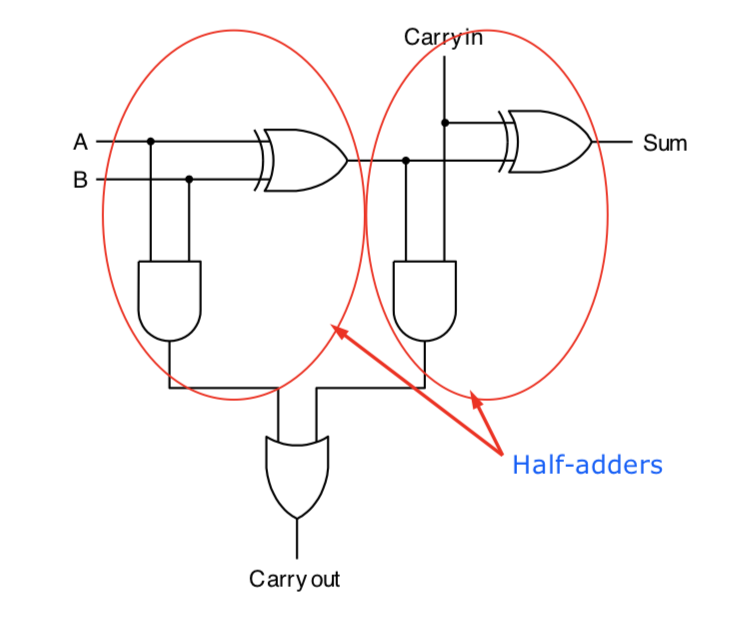
\includegraphics[width=0.8\linewidth]{fulladder}	
\end{figure}


\subsection{Binary Adder}
Can cascade full adders to make binary adder. This is a \textbf{ripple-carry adder}.
\begin{figure}[H]
	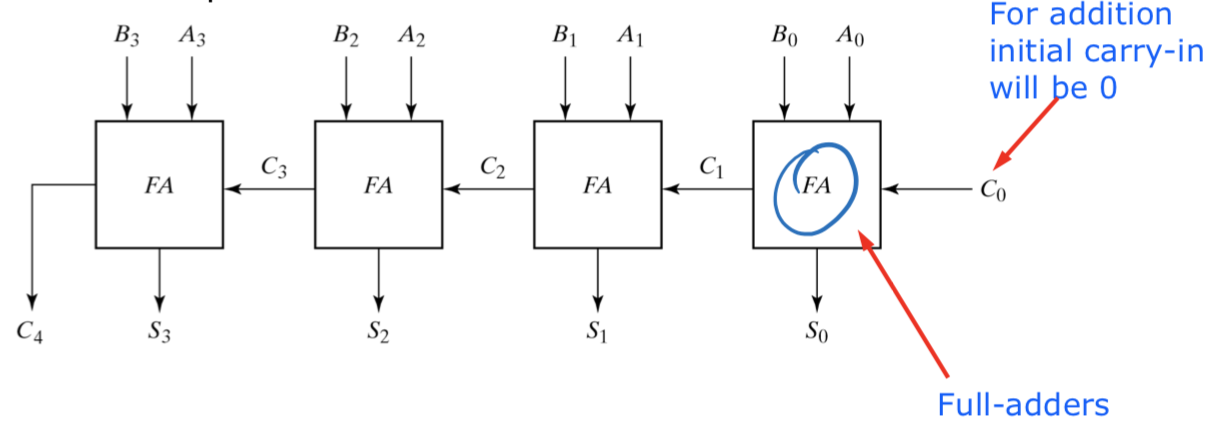
\includegraphics[width=0.8\linewidth]{binaryadder}	
\end{figure}



%\begin{circuitikz}
%	\draw (1, -2) node [and port,rotate=-90] (and1) {};
%	\draw (5, -2) node [and port,rotate=-90] (and2) {};
%	\draw (3, -4) node [or port,rotate=-90] (or1) {};
%	\draw (and1.out) |- (or1.in 2);
%	\draw (and2.out) |- (or1.in 1);
%	
%	\draw (3, 0.5) node [xor port] (xor1) {};
%	
%	\draw (0, 0) node (a) {A};
%	\draw (0, 1) node (b) {B};
%	
%	\draw (a) -| (and1.in 1);
%	\draw (a) -| (xor1.in 2);
%	\draw (b) -| (and1.in 2);
%	\draw (b) -| (xor1.in 1);
%\end{circuitikz}

% !TeX spellcheck = en_US
% !TeX root = notes.tex
\section{Combination Logic}
\subsection{Combinational Circuits}
Each output can be expressed as a function of $n$ input variables. Can write truth table also:
\begin{itemize}
	\item $n$ input columns
	\item $m$ output columns
	\item $2^n$ rows (i.e. possible input combination)
\end{itemize}

\begin{note}{Multiplexer (or Mux)}
	\begin{itemize}
		\item $2^n$ data inputs
		\item 1 output
		\item $n$ control (or \textbf{select}) inputs - that \textbf{select} one of the inputs to be ``sent'' or ``steered'' to the output	
	\end{itemize}
\end{note}

\begin{note}{Decoder}
	Converts $n$-bit input to a logic-1 on exactly one of $2^n$ outputs	
\end{note}

\subsection{Timing Diagram}
\begin{figure}[H]
	\begin{tikztimingtable}[timing/slope=0,timing/coldist=2pt,xscale=4,semithick]
		Input & LHL \\
		Output & HLH \\
		\extracode\makeatletter
		\begin{pgfonlayer}{background}
			\begin{scope}[gray,semitransparent,semithick]
				\horlines{}
				\vertlines{0,...,3}	
			\end{scope}
		\end{pgfonlayer}
	\end{tikztimingtable}
	\centering\caption{Timing Diagram of an inverter}
\end{figure}

There is a slight delay in logic timings in reality
\begin{figure}[H]
	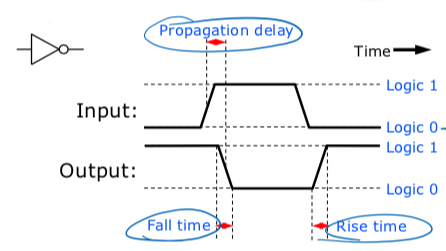
\includegraphics[width=0.8\linewidth]{timing}
	\centering\caption{Reality of Timing}
\end{figure}
\begin{description}
	\item[Propagation delay:] time for change in input to affect output
	\item[Fall time:] time taken for output to fall from 1 to 0
	\item[Rise time:] time for output to rise from 0 to 1	
\end{description}





\end{multicols*}
\end{document}
